\section{Описание прототипа}\label{prototype}

В описании к авторскому свидетельству №844986, кл. G 01 B 7/06 (по заявке №4822394/28 от 22.03.90 г., автор В.Г.Панов) представлено устройство \glqq Емкостной датчик микроперемещений\grqq, функциональная схема которого приведена на рисунке~\ref{schema}.

\begin{figure}[h]
	\centering
	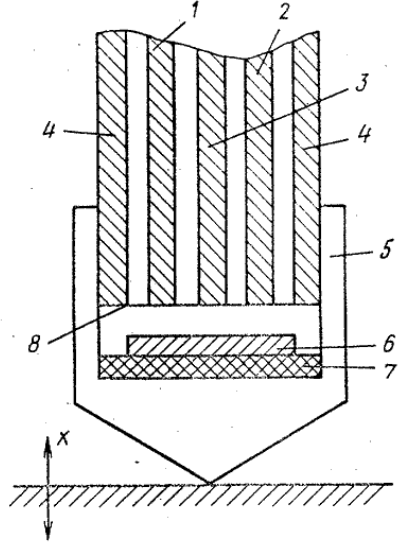
\includegraphics[width=0.4\textwidth]{schema.png}
	\caption{Функциональная схема датчика}
	\label{schema}
\end{figure}

Датчик содержит неподвижные потенциальный $1$ и измерительный $2$ электроды и охватывающие их внутренний $3$ и внешний $4$ экраны. Торцы электродов и экранов лежат в рабочей плоскости датчика. Снаружи боковой цилиндрической поверхности внешнего экрана $4$ размещен с возможностью возвратно- поступательного движения щуп $5$, во внутренней полости которого размещена металлическая пластина $6$, которая электрически изолирована от корпуса датчика и расположена параллельно рабочей плоскости его электродов и экранов. При перемещении щупа $5$ изменяется зазор между пластиной $6$ и рабочими торцами электродов и экранов, что приводит к изменению емкости датчика.

Датчик работает следующим образом: при перемещении объекта изменяется воздушный зазор между плоскостью металлической пластинки $5$ и рабочей плоскостью $8$ 
электродов $1$ и $2$ и экранов $3$ и $4$ датчика, вследствие чего изменяется выходное напряжение $U_{\text{вых}}$, снимаемое с измерительного электрода $2$ датчика. Чувствительность датчика зависит от величины диэлектрической постоянной материала контролируемого объекта и максимальна в диапазоне $0 - x_{\text{мин}}$, где $x_{\text{мин}}$~-- величина микроперемещения, когда металлическая пластина $6$ не заземлена. Герметизация щупа $5$ позволяет свести к минимуму погрешности, связанные с влиянием внешних условий.


\begin{figure}[h]
	\centering
	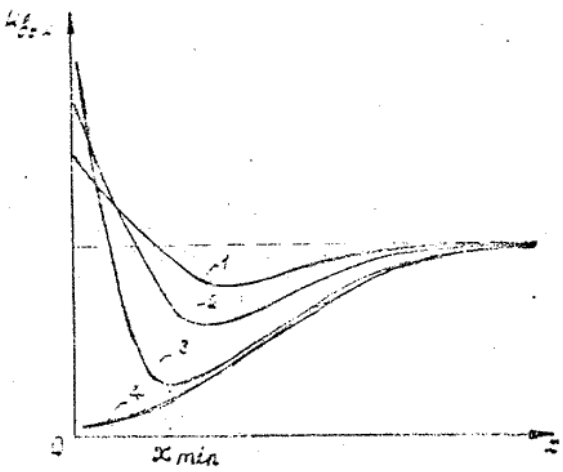
\includegraphics[width=0.4\textwidth]{out.png}
	\caption{Выходная характеристика в зависимости от диэлектрической проницаемости}
	\label{out}
\end{figure}


\section{Анализ и синтез по закону полноты частей системы}

Закон формулируется следующим образом: необходимым условием
принципиальной жизнеспособности ТС является наличие и минимальная
работоспособность основных частей системы. Таких основных частей
четыре: двигатель (Дв), трансмиссия (Тр) или передача, рабочий орган (Ро) и орган управления (Оу).

Определим основные части системы, представленной на рисунке~\ref{schema}. Сначала, определим рабочий орган -- Ро. Датчик предназначен для измерения расстояния. Расстояние выражается в изменении емкости между рабочей плоскостью 8 и пластиной 6. Изменение емкости влияет на выходное напряжение, которое измеряется при помощи с <<конденсатора>>, образованного следующими элементами потенциальным электродом 1, пластиной 6 и измерительным электродом 2. 

Далее определим двигатель как часть системы, вырабатывающей энергетику. Здесь двигателем является балка, в которую упирается щуп 5. Тогда трансмиссией являются щуп, подложка 7 и пластина 6. Органов управления в рассматриваемом датчике нет, поэтому система является неполной. Структурная схема представлена на рисунке~\ref{first_sys}

\begin{figure}[h]
	\centering
	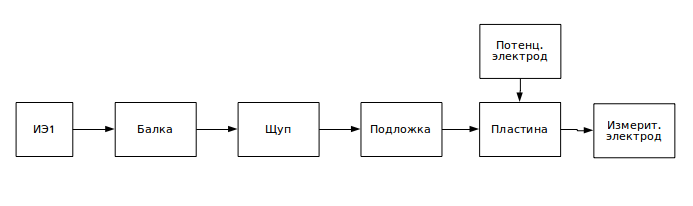
\includegraphics[width=1\textwidth]{pic0.png}
	\caption{Структурная схема рассматриваемой системы}
	\label{first_sys}
\end{figure}

Чтобы получить новые технические решения с использованием закона полноты частей  системы, можно добавить недостающие элементы в систему. 

Каждая ТС должна включать четыре части: двигатель, трансмиссию, рабочий орган и орган управления. Для синтеза ТС необходимо наличие этих четырех частей и их минимальная пригодность к выполнению функций системы.

Добавим в систему орган управления (ОУ) и измерительную часть -- мостовую схему измерения, представленную на рисунке~\ref{im:bridge}, где $C_x$~-- представление датчика, как переменный конденсатор, $R_1$ и $R_2$~-- резисторы, У~-- усилитель, ИБ~-- измерительный прибор. Переменный конденсатор $C_3$, при помощи которого сможем подстраивать нулевое положения датчика. Этот конденсатор будет выступать в качестве Органа управления.


\begin{figure}[h]
	\centering
	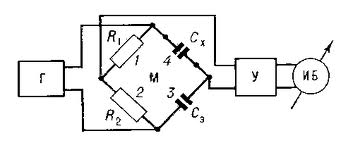
\includegraphics[width=0.6\textwidth]{bridge.jpg}
	\caption{Схема измерения емкости датчика с подстройкой}
	\label{im:bridge}
\end{figure}


\begin{figure}[h!]
	\centering
	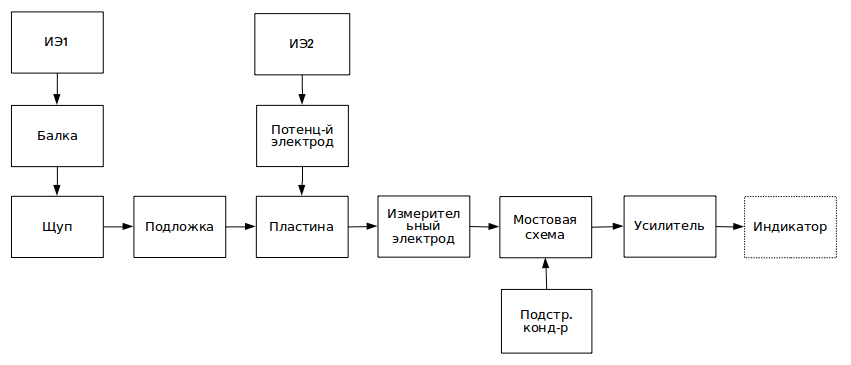
\includegraphics[width=1\textwidth]{pic1.png}
	\caption{Структурная схема полной системы}
	\label{pic1}
\end{figure}

Чтобы получить новые технические решения с использованием закона полноты частей системы, можно использовать линию на вытеснение человека из ТС. В соответствии с
линией вытеснения действия человека необходимо искать на окончании этой линии -- в органах управления.

В рассматриваемой системе балка давит на щуп, который в свою очередь это давление передает через подложку 7 на пластину 6. Пластина шесть изменяет свое положение относительно плоскости электродов 8. Электроды и пластина, образующие конденсатор, емкость которого изменяется, в результате чего с измерительной схемы на усилитель передается отклонение пластины от нулевого положения, заданного человеком при помощи подстроечного конденсатора. Для вытеснения этой функции человека этот конденсатор должен подстраиваться автоматически при включении системы. Нужно заменить конденсатор на устройство подстройки емкости, при помощи подачи некоторого информационного сигнала 
с надсистемы.

Система получается с автоматической калибровкой. Такая система обладает меньшими ошибками и более простой в использовании. 

Таким образом, с точки зрения закона получили полную систему.


\section{Анализ и синтез по закону энергетической и информационной проводимости ТС}

Закон формулируется следующим образом: необходимым условием
принципиальной жизнеспособности ТС является сквозной проход энергии
и информации по всем частям технической системы.

Проанализируем систему с рисунка~\ref{pic1} по закону энергетической проводимости. Построение линии начнем с ИП, рисунок~\ref{im:bridge}, он выделяет электрическую энергию. Электрическое поле ИП воздействие на потенциальный электрод, на выходе которого формируется напряжение. Информативный параметр электрического поля в данном случае -- это переменное напряжения. 
Поле давления действует на щуп, в результате чего он изменяет свое положение относительно корпуса. 
Поле давления от щупа воздействует на подложке. Поле давления от подложки воздействует на пластину. Электрическое поле от потенциального электрода воздействует на пластину. Электрическое поле от пластины воздействует на измерительный электрод. Электрическое поле от Измерительного электрода воздействует на Мостовую измерительную схему. Информационным параметр электрического поля в этом случае -- это рассогласование емкости эталонного конденсатора и емкости между электродами и пластиной. Поле электрического поля от мостовой схемы воздействует на усилитель. Выходным информационным параметром усилителя будет напряжение.


\begin{figure}[h!]
	\centering
	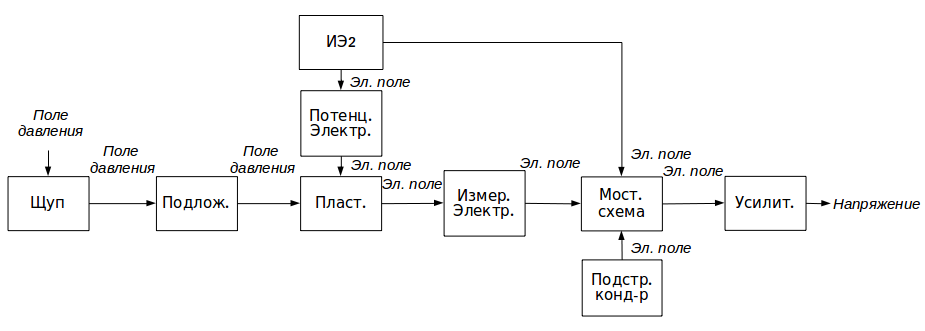
\includegraphics[width=1\textwidth]{energy.png}
	\caption{Линия прохода энергии и информации}
	\label{}
\end{figure}

Для синтеза новых решений можно замкнуть линию прохождения энергии, получив кольцо. 

По этому закону можно дополнить систему на входе регулятором и пьезодвигателем, поле давление которого будет воздействовать на щуп. Для этого выход усилителя замкнем на вход регулятора, напряжение которого будем подавать на пьезодвигатель.

\begin{figure}[h!]
	\centering
	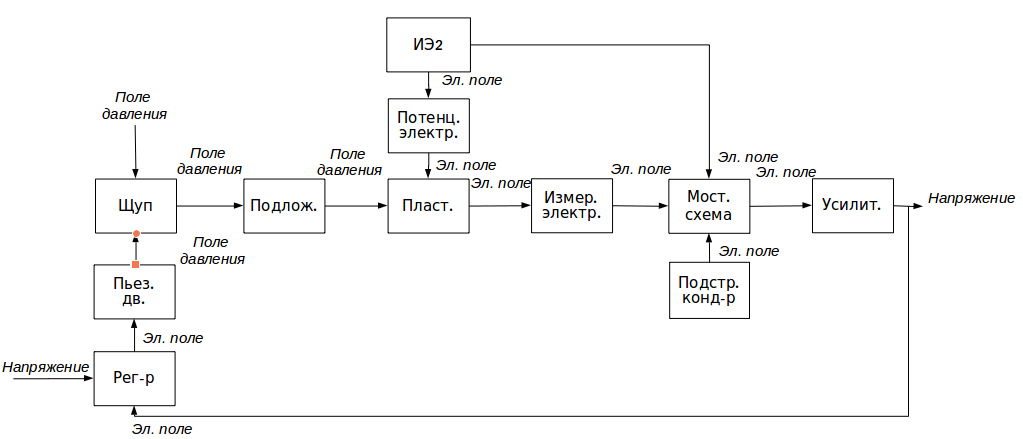
\includegraphics[width=1\textwidth]{cloe_loop.png}
	\caption{Линия прохода энергии и информации в замкнутой схеме}
	\label{sogl1}
\end{figure}

\section{Закон согласования-рассогласования технических систем}

Составляющие техническую систему части должны быть согласованы или, наоборот, рассогласованы между собой.

Например, для согласования параметров входной физической величины и выходной электрической служит Пластина 6.

С точки зрения этого закона можно проверить согласованность по темпам протекания процессов, происходящих в основных частях системы.

Система рассогласована по темпам протекания процессов. Изменение расстояния между пластиной и плоскостью электродов, происходит медленнее, чем протекают токи в электрических схемах мостовой схемы и усилителя. Чтобы согласовать ее, можно заменить электрическую часть механической, в которой перемещение щупа через механические передачи будет преобразовываться в показания стрелочного индикатора.

С точки зрения энергетических параметром, полученная система на рисунке~\ref{sogl1} согласована по входным и выходным информационным сигналам.

Система рассогласована в части параметров материалов. Для согласования системы, чтобы избавиться от вредного явления трения между корпусом и щупом, а в перспективе и износа щупа, можно убрать щуп.
\begin{figure}[h!]
	\centering
	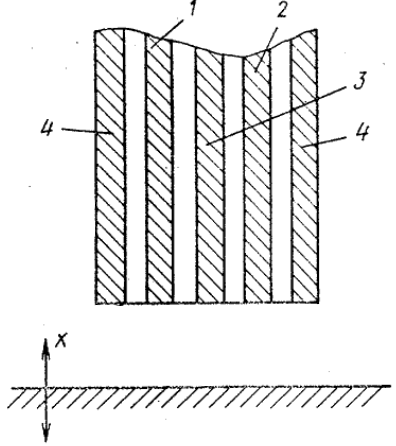
\includegraphics[width=0.5\textwidth]{new1.png}
	\caption{Емкостной датчик расстояния без щупа}
	\label{sogl1}
\end{figure}


\section{Анализ и синтез систем по закону увеличения степени идеальности}

Закон увеличения степени идеальности является одним из основных законом развития ТС. Под увеличением степени идеальности И в ТРИЗ понимается рост отношения суммы выполняемых системой полезных функций Фп к сумме факторов расплаты Фр.

Для повышения степени идеальности путем увеличения числителя формулы необходимо возложить на систему еще одну или несколько функций, ранее ею не выполнявшихся. Например, при добавлении обратной связи, позволяющей стабилизировать конструкцию в зависимости от выходного напряжения получаем новое устройство -- стабилизатор заданного расстояния. 

Факторами расплаты в этом случае будут являться добавление новых элементов в систему, таких как пьезодвигатель и регулятор. 

При добавлении пружины в датчик, таким образом уменьшив инерционность щупа, датчик получает новую функцию измерение вибраций.

Датчик без щупа может быть использован в качестве бесконтактного выключателя в емкости с жидкостью или сыпучими материалами.

\begin{figure}[h!]
	\centering
	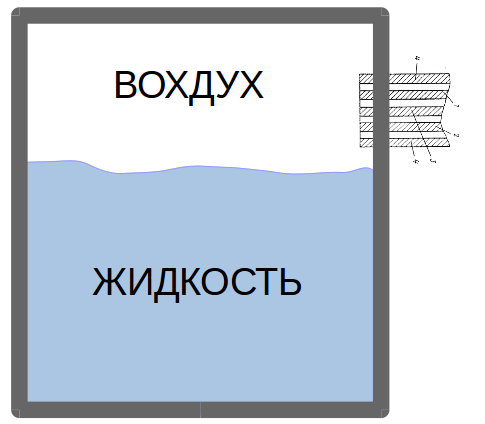
\includegraphics[width=0.5\textwidth]{new2.png}
	\caption{Новая функция -- определение уровня жидкости}
	\label{sogl3}
\end{figure}

Попробуем уменьшить знаменатель. Для этого исключим из системы какую-либо её часть, например, уберем щуп -- расстояния измерять все еще можно, но в системе появляются электромагнитные помехи.

\section{Закон неравномерного развития технических систем}

В процессе количественного роста в результате неравномерного развития характеристик технической системы появляются противоречия, происходит накопление и обострение противоречий.

Выберем содержательную характеристику, которую будем улучшать, т.е. цель. Расширим диапазон измерения датчика. Чтобы измерять большие расстояния, нужно увеличивать зазор между пластиной и электродами. Но при увеличении расстояния уже хотябы на сантиметр, датчик оказывается неработоспособным. Возникает противоречие: пластина должна отодвигаться от плоскости электродов на большое расстояние и, одновременно, на небольшое, чтобы датчик был работоспособен.

Разрешим это противоречие с помощью алгоритма решения изобретательских задач (АРИЗ).


\begin{enumerate}[1]
	\item Анализ задачи
	\begin{enumerate}
	\item Модель задачи
		
		Имеем техническую систему для измерения перемещений, которая включает корпус, щуп, измерительный и потенциальный электроды, внутренний и внешний экраны, подложку, пластину, мостовую схему и усилитель. Обратная связь по выходному напряжению, регулятор и пьезоэлектрический двигатель.
		
		Технической противоречие (ТП): пластина должна быть на большом расстоянии от плоскости электродов и на маленьком, чтобы датчик оставался роботоспособным.
		
		\item Выбор конфликтной пары
		
		Инструмент: пластина. Изделие: плоскость электродов и электрическое поле.
		
		\item Составление схемы технического противоречия 
		
		\begin{figure}[h!]
			\centering
			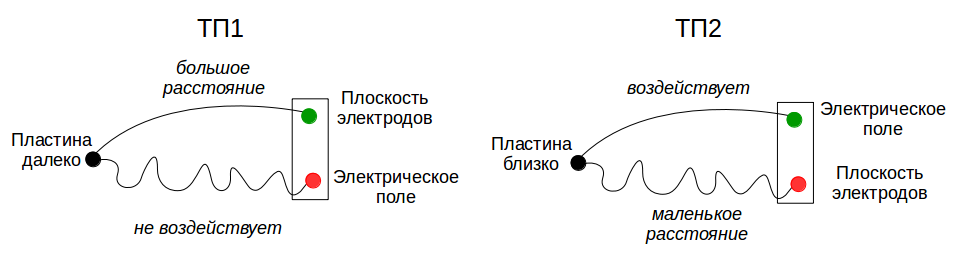
\includegraphics[width=1\textwidth]{tp.png}
			\caption{Граф-схема технического противоречия}
			\label{tp}
		\end{figure}
		
		\item Выбор ТП1, так как необходимо увеличить измеряемое расстояние.
		\item Усиление конфликта
		
		Выбираем большое расстояние между пластиной и плоскостью электродов, например, 0.1 м.
		\item Модель решения
		
		Дана техническая система для измерения расстояний порядка сантиметров. Когда пластина далеко от плоскости с электродами, то датчик имеет широкий диапазон измерения расстояний, но при этому электрическое поле не позволяет измерить емкость между пластиной и электродами на большом расстоянии.
		
		Необходимо ввести $\textbf{x}$-элемент, который позволит электрическому полю воздействовать на пластину на любом расстоянии в пределах требуемого диапазона измерений.	
	\end{enumerate}
	\item Анализ модели задачи
	\begin{enumerate}
		\item Определение оперативной зоны (ОЗ)	
		
		Воздушное пространство между пластиной и плоскостью электродов.
		\item Определение оперативного времени (ОВ)
		
		В качестве оперативного времени выберем время конфликта, т.е. то время, когда на пластину не действует электрическое поле от электродов.
		\begin{equation}
		T = T_1 + T_2 + T_3
		\end{equation}
		где $T_1$~--- время конфликта, $T_2$~--- сам конфликт, $T_3$~--- время после конфликта.
		
		\item Анализ вещественно-полевых ресурсов (ВПР)
		
		Внутрисистемные:
		Инструмент: вещество (Пластина). Габариты, геометрическая форма, материал.
		
		Изделие: вещество (корпус с электродами) и электрическое поле.
		
		Внешнесистемные: Помехи от бытовой электотехники, пыль, вода, изменение характеристик воздуха.
		
		Надсистемные: гравитационное, магнитное поле Земли.
		
	\end{enumerate}	
	
	\item Идеальный конечный результат и физические противоречия
	\begin{enumerate}
		\item Предварительный ИКР (ИКР1)
		
			Икс-элемент, абсолютно не усложняя систему и не вызывая вредных явлений, устраняет недостижимость электрического поля пластины в течение оперативного времени (ОВ) 	в пределах оперативной зоны (ОЗ), сохраняя способность инструмента совершать измерение расстояния.
		
		\item Усиленный ИКР

			Заменим икс-элемент словом пластина. Можно изменить параметры пластины таким образом, чтобы на нее всегда действовало электрическое поле.
			Можно ввести такую среду, которая будет передавать электрическое поле от корпуса к пластине.

		\item Физические противоречия на макроуровне
		
			Противоречие икс-элемент должен быть одновременно длинным, чтобы доставать до корпуса и не должен быть длинным, чтобы быть в диапазоне измерения емкости.

		\item Физические противоречия на микроуровне

			В оперативной зоне должны быть частицы вещества сильно подвижные, чтобы обеспечить перемещение на большое расстояние, и не должны быть такие частицы, чтобы обеспечить пропорциональное изменение емкости.
	\end{enumerate}

	\item Метод маленьких человечков

Обозначим частицы икс-элемента в виде меленьких человечков. Тогда, чтобы обеспечить связь пластины и электродов заполним пространство между ними маленькими человечками. В первом случае человечки это частицы воздуха, они не могут передавать электрическое поле от электродов к пластине. Освободим руки человечков, чтобы они могли передавать электрическое поле пластине. Для этого нужно заполнить пространство между пластиной и корпусом веществом, которое сможет влиять на электрическую емкость при изменении расстояния между пластиной и корпусом. Возьмем пористый материал, который при сжимании меняет свою плотность и, соответственно, диэлектрическую проницаемость, например губка. Задача решена. 

\begin{figure}[h!]
	\centering
	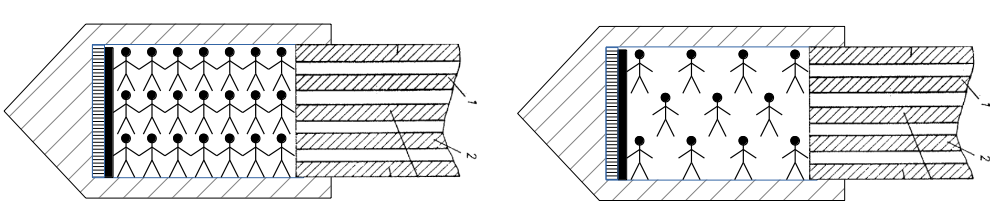
\includegraphics[width=1\textwidth]{new4.png}
	\caption{Рисунок ММЧ}
	\label{new4}
\end{figure}

\end{enumerate}
\newpage
\subsection{Вепольный анализ}

Система должна образовывать полный веполь. Найдем в исходной ТС неполный веполь и сделаем его полным.

Пусть В1~-- пластина, П~-- неохватывание электрическим поле пластины. При отдалении пластины от корпуса с электродами, электрическое поле перестает воздействовать на платину.

\begin{figure}[h!]
	\centering
	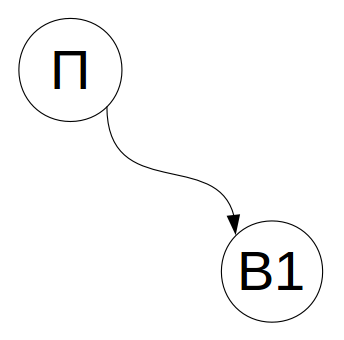
\includegraphics[width=0.4\textwidth]{new5.png}
	\caption{Неполный веполь}
	\label{new5}
\end{figure}

Чтобы система стала полным веполем, введем В2~-- вещество, которое должно устранить вредное воздействие П на В1.

\begin{figure}[h!]
	\centering
	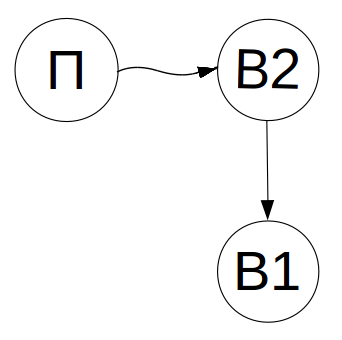
\includegraphics[width=0.4\textwidth]{new6.png}
	\caption{Полный веполь}
	\label{new6}
\end{figure}
\newpage
Вторым веществом В2, которое позволяет сохранить связь между перемещением пластины и электрическим током является пористая губка. Это сохраняет зависимость между перемещением пластины и изменением емкости в поле действия электродов

\subsection{Морфологический анализ}

Составим таблицу, в которой укажем элементы исходной ТС и их свойства.

\begin{table}[h!]
	\centering
	\caption{Морфологический анализ}
	\label{morph}\scriptsize
	\begin{tabular}{|l|c|c|c|c|c|c|}
		\hline
		\multicolumn{1}{|c|}{}          & \textbf{Твердый} & \textbf{Лег-й} & \textbf{Элект-ый} & \textbf{Магнит-ый} & \textbf{Подвижн.} & \textbf{Наст-ый} \\ \hline
		\textbf{Корпус}                 & +                & -               & -                          & -                          & -                  & -                      \\ \hline
		\textbf{Щуп}                    & +                & +               & +                          & -                          & +                  & -                      \\ \hline
		\textbf{Подложка}               & +                & +               & -                          & -                          & +                  & -                      \\ \hline
		\textbf{Пластина}               & +                & +               & +                          & -                          & +                  & -                      \\ \hline
		\textbf{Измерительный электрод} & +                & -               & +                          & -                          & -                  & -                      \\ \hline
		\textbf{Потенциальный электрод} & +                & -               & +                          & -                          & -                  & -                      \\ \hline
		\textbf{Внутренний экран}       & +                & -               & +                          & -                          & -                  & -                      \\ \hline
		\textbf{Вешний экран}           & +                & -               & +                          & -                          & -                  & -                      \\ \hline
		\textbf{Мост. Схема}            & -                & -               & +                          & -                          & -                  & +                      \\ \hline
		\textbf{Усилитель}              & -                & -               & +                          & -                          & -                  & -                      \\ \hline
		\textbf{Конденсатор}            & -                & -               & +                          & -                          & -                  & +                      \\ \hline
	\end{tabular}
\end{table}
\normalsize

Из анализа таблицы получаем $11 \times 6 = 66$ вариантов возможного исполнения устройства. По количеству <<$+$>> определяем варианты реально имеющихся устройств: $24$. По количеству <<$-$>> определяем максимально возможное количество новых изобретений, полученных в результате анализа: $42$. 

Можно составить новые технические решения на основании таблицы~\ref{morph} 

Приведем новые технические решения на основе следующих пар, имеющих знак <<$-$>>:
\begin{enumerate}
	\item Настраиваемый пластина. Новое техническое решение: изменение площади пластины в электрическом поле электродов при ее повороте позволит измерять угол поворота.
	\item Подвижный измерительный электрод. Вкручивая и выкручивая его в корпус можно подстраивать емкость под эталон. Таким образом можно избавиться от подстроечного конденсатора.
	\item  Электропроводный корпус. Можем отказаться от специальных экранов, а электроды провести через отверстия сквозь корпус в изоляции.
	\item Настраиваемый щуп. Разная форма и исполнение щупа позволят расширить круг задач, для которых применяется полученное устройство. Например, щуп удлинитель.
\end{enumerate}

\subsection{Формула учебного изобретения}

Емкостной датчик перемещений, состоящий из корпуса с двумя потенциальным и измерительным электродами для измерения емкости между ними, щупа, пластины, размещенной в щупе на диэлектрической подложке, параллельно плоскости электродов. Электроды в корпусе изолированы друг от друга внутренним экраном и оба изолированы от внешних электромагнитных полей внешним экраном. Отличается тем, что между пластиной и плоскостью находится пористая губка.

\section{Закон повышения динамичности и управляемости ТС}

Закон заключается в том, что в процессе развития ТС повышается способность ее к целенаправленным изменениям, обеспечивающим наилучшее приспособление к изменяющейся внешней среде.

По этому законом можно ввести обратную связь по положению щупа в результате чего получится стабилизирующаяся конструкция.

Определим неподвижные (статичные) части системы и сделаем их динамичными для повышения динамичности и управляемости.

Добавив возможность сменять щупы разной конструкции, придадим более широкий круг применения датчику.

Добавив возможность перемещения пластины в щупе, приобретем регулировку диапазона измерения.

Если щуп сделать несимметричным и позволить ему вращаться вокруг корпуса, то это позволит измерять как линейные перемещения, так и угловые.
 
\section{Закон развертывания-свертывания}

Повышение идеальности ТС осуществляется путем развертывания --  увеличения количества и качества выполняемых функций, приносящих пользу, но за счет увеличения сложности системы, и свертывания -- упрощения системы при сохранении или увеличении количества и качества полезных функций. 

Свертывание системы происходит при анализе и синтезе системы по закону увеличения степени идеальности, где мы отказываясь от щупа, получаем возможность измерять емкость среды в поле действия электрического поля электродов.

Развертывание системы проявляется при анализе и синтезе по закону энергетической и информационной проводимости, когда мы добавляем в систему вещества и поля, чтобы обеспечить сквозной проход энергии и информации по всем частям ТС.

\section{Закон перехода на микроуровень и использование полей}

Переход на микроуровень - это основной путь свертывания ТС,
вообще развитие техники в целом идет в направлении все большего
использования глубинных уровней строения материи.

С точки зрения этого закона емкостной датчик перемещений находится на первом уровне, так как содержит элементы простой специальной формы -- стержни (электроды), пластины.

Для перехода на микроуровень можно добавить демпфирующую пружину к щупу. Что придаст систему нечувствительность к небольшим колебаниям.

\section{Статическая модель технического противоречия}

Для моделирования из таблицы канонических катастроф выбираем катастрофу типа «сборка», так как в модели имеется два состояния устойчивого равновесия ТП1 и ТП2

Этой катастрофе соответствует потенциальная функция:
\begin{equation}
	E(x) = 0.25 x^4 - 0.5 \lambda x^2 - \mu x
\end{equation}
где $x$~-- состояние инструмента (пластина), $E(x)$~-- характеризует удаление пластины от корпуса с электродами.

Пусть, у прототипа максимальное отклонение $E(x) = c = const = 10$ см. Выберем начальное расстояние между пластиной и корпусом равным $10$ см.

Запишем потенциальную функцию для нашей задачи с учетом того, что любая потенциальная функция определяется с точностью до константы $c$
\begin{equation}
	E(x) = 0.25 (x-10)^4 - 0.5 \lambda (x-10)^2 - \mu (x-10) + c	
\end{equation}

Так как размерности $x$ м и $E(x)$ см, то коэффициент пропорциональности $d = 0.01$.

Допустим исходное положение пластины $x =10$ см, тогда $E(x) = 10$ см.

Пусть $D_{min}=3$ м -- малое расстояние между пластиной и корпусом, $D_{max} = 7$ м -- большое расстояние.  Тогда мощность конфликта можно рассчитать, как
\begin{align}
	D_{max} - D_{min} = 2 \sqrt{\lambda} = 16\\
	\lambda = 0.25 (D_{max} - D_{min})^2 = 4
\end{align}

Для усиления конфликта, пусть $D_{min}=0.1$ м -- наименьшее расстояние между пластиной и корпусом, $D_{max} = 9.9$ м -- наибольшее расстояние.  Тогда мощность конфликта
\begin{align}
D_{max} - D_{min} = 2 \sqrt{\lambda} = 9.8\\
\lambda = 0.25 (D_{max} - D_{min})^2 = 24.01
\end{align}

Предположим, что для этой мощности конфликта находим решение задачи, т.е. $x$-элемент. Найдем критическое значение параметра $\mu$, задающего величину $x$-элемента по формуле 
\begin{equation}
	\mu_{\text{кр}}  = \pm \cfrac{2 \lambda}{3} * \sqrt{\cfrac{\lambda}{3}} = \pm \cfrac{2 * 24.01}{3} * \sqrt{\cfrac{24.01}{3}} = \pm 45.28 cm^3
\end{equation}

Допустим, что диапазон расстояний достаточно велик. Тогда знак параметра будет положительным, т.е. $\mu = 45,28$ см$^3$. Также будем считать, что в результате решения задачи рабочий диапазон уменьшился до $E(x)=7$ см.

Графики потенциальной функции для всех трех случаев набора управляющих параметров изображены на рисунке~\ref{potenc}. 

\begin{figure}[h!]
	\centering
	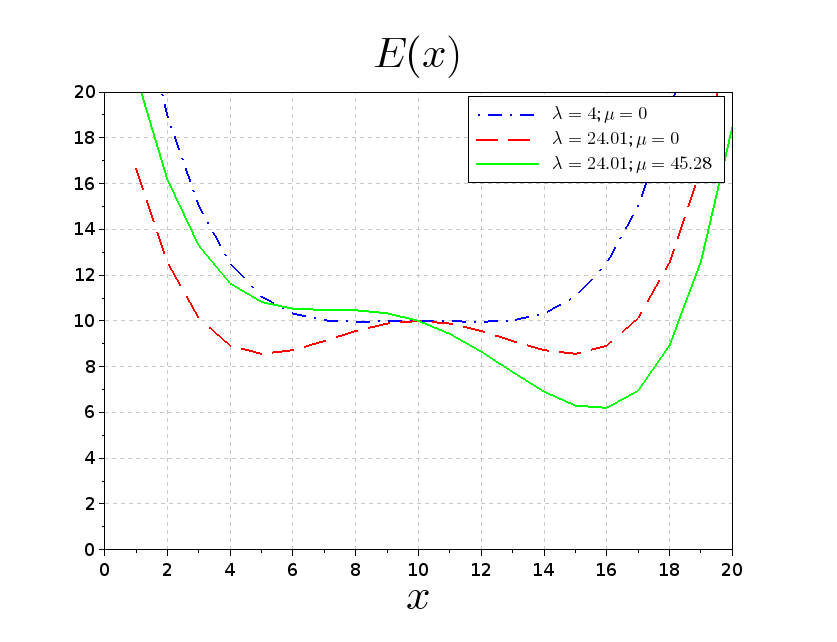
\includegraphics[width=1\textwidth]{potenc.png}
	\caption{Графики перемещения пластины}
	\label{potenc}
\end{figure}

Графики отражают изменение расстояния между пластиной и корпусом с электродами.
Окончательное решение задачи моделирует график с $\lambda = 24.01 cm^2$ т $\mu = 45.28 cm^2$.
\newpage
Из этого графика видно, что при таком выборе управляющих параметров $\lambda$ и $\mu$, а также масштабирующего коэффициента d, перемещение пластины равно $6.1$ cm. 

\newpage
\section{Одномерная динамическиая модель технического противоречия}

Для нашего примера статической модели запишем потенциальную функцию в общем виде:
\begin{equation}
	E(x) = 0.25 (x-10)^4 - 0.5 \lambda (x-10)^2 - \mu (x-10) + c
\end{equation}

Возьмем от нее производную по $z$, где для простоты моделирования
принято $z = x-10$. Получим градиент
\begin{equation}
	\cfrac{\partial E}{\partial z} = (z^3 - \lambda z^2 - \mu)d
\end{equation}

Приравняем антиградиент производной $\cfrac{\partial z}{\partial t} $ коэффициентом пропорциональности $CT$
\begin{equation}
	\cfrac{- \partial E}{\partial z} = - (z^3 - \lambda z^2 - \mu)d = CT \cfrac{\partial z}{\partial t} = CT \dot z
\end{equation}
где $T$~--- постоянная времени психологической инерции решателя задачи, $T = 1, C = d$.

Тогда получаем стандартное уравнение 
\begin{equation}
	\dot z = -z^3 + \lambda z + \mu
\end{equation}
где значения $\lambda$ и $\mu$ выбираем равными значениям, полученным в статической модели.

\begin{figure}[h!]
	\centering
	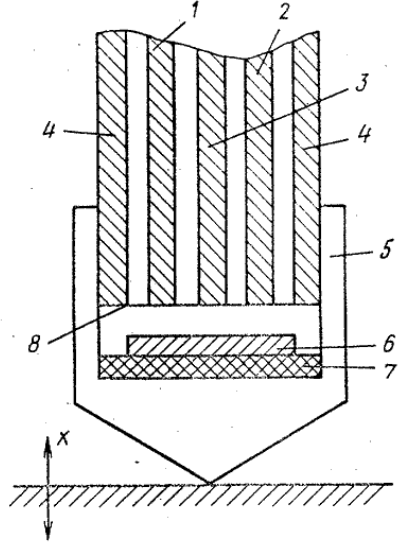
\includegraphics[width=0.7\textwidth]{schema.png}
	\caption{Схема динамической модели}
	\label{schema}
\end{figure}
Запишем уравнения для состояния равновесия:
\begin{equation}
	u = z^3 - z
\end{equation}
\begin{equation}
	z = f - K u
\end{equation}
Подставляя значения $u$ из первого уравнения во второе, получаем:
\begin{equation}
	-z^3 + \cfrac{K-1}{K}z + \cfrac{f}{K} = 0
\end{equation}

Сравнивая полученное уравнение с уравнением «сборки», определяем, что:
\begin{align}
	\lambda = \cfrac{K-1}{K}\\
	\mu = \cfrac{f}{K}
\end{align}

Рассчитываем $K$ и $f$
\begin{align}
	K = \cfrac{1}{1-\lambda} = - 0.0434\\
	f = K \mu =- 1.9679 
\end{align}

Строим кривую катастроф
\begin{align}
	f = \pm \cfrac{2 \sqrt{3}}{9} (K-1) \sqrt{\cfrac{K-1}{K}} = 1.986322 
\end{align}

\begin{figure}[h!]
	\centering
	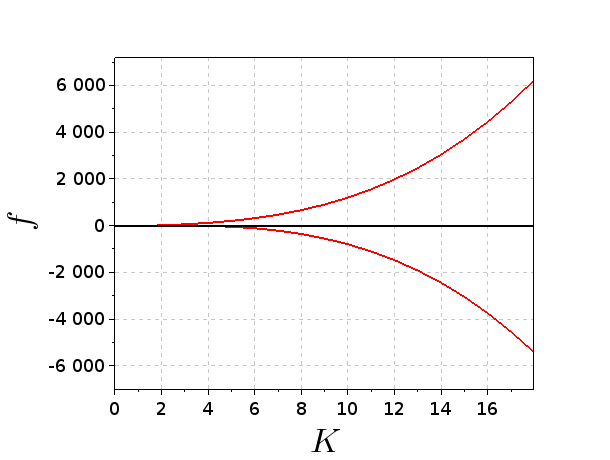
\includegraphics[width=0.7\textwidth]{fk.png}
	\caption{Кривая катастроф}
	\label{aaa}
\end{figure}

Для удобства получения дифференциального уравнения, описывающего схему моделирования в форме Коши, апериодическое звено в схеме на рисунке~\ref{schema}представим виде эквивалентной схемы: интегратора, охваченного обратной связью.

\begin{figure}[h!]
	\centering
	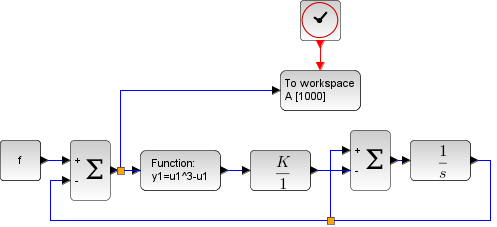
\includegraphics[width=0.7\textwidth]{scheama4.png}
	\caption{Схема моделирования в нормальной форме Коши}
	\label{aaa}
\end{figure}

Для моделирования при двух устойчивых состояниях равновесия найдем область начальных условий на координату $z$, для установки в интегратор схемы моделирования. Область устойчивости определяется из уравнения:

\begin{align}
(1-3 z^2 - 3 f^2 + 6 f z) K - 1 < 0
\end{align}

Так как значение $\mu$ должно быть по модулю меньше критического пересчитаем значение для $f$, предварительно выбрав $\mu = \cfrac{\mu_{\text{крит}}}{2} = 23.34$. Тогда

\begin{align}
	f = K \mu = - 0.99
\end{align}

Находим границы областей устойчивости, подставив выбранные значения в формулу для определения устойчивости, приравняв правую часть нулю:


\begin{align}
	(1-3 z^2 - 3 (-0.99)^2 + 6 (-0.99) z)  (-0.0425) - 1 = 0
\end{align}

Находим корни, задающие границы устойчивости
\begin{align}
	z_1 = - 3.835;\\
	z_2 = 1.87
\end{align}

Наносим границы на фазовом портрете системы, который строится по уравнению
\begin{align}
	\dot z = z - K ((f-z)^3 - (f-z)) = z + 0.0425 ((-0.99 - z)^2 -(-0.99 - z)) 
\end{align}

Приравниваем нулю производную для получения уравнения установившегося режима

\begin{align}
	z_s + 0.0425 ((-0.99 - z_s)^2 -(-0.99 - z_s)) = 0
\end{align}

Находим корни
\begin{align}
	z_{s1} = - 6.36;\\
	z_{s2} = -0.00009;\\
	z_{s3} = 3.39
\end{align}


\begin{figure}[h!]
	\centering
	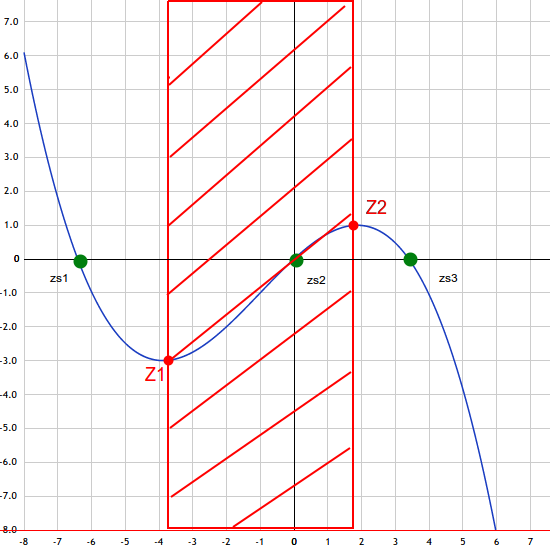
\includegraphics[width=0.5\textwidth]{graph.png}
	\caption{Фазовый портрет системы}
	\label{aaa}
\end{figure}


Первый и третий корни принадлежат к области устойчивости, т.е. являются точками устойчивого равновесия, а второй корень принадлежит к области неустойчивости, т.е. является точкой неустойчивого равновесия. Это видно из фазового портрета системы, где область неустойчивости определяется корнями  и заштрихована.
Подставляя найденные значения в схему моделирования, получаем модель в виде, представленном на рисунке~\ref{schema}. Удобнее всего моделировать процесс сразу же с двух разных начальных условий. Для этого набирается два абсолютно одинаковых канала, но с разными начальными условиями на интеграторы. 
Выбираем начальные условия на интегратор из области притяжения одного из устойчивых корней, например, $z(0)=-5$ и из области притяжения другого корня, например, $z(0)=1$ и получаем переходный процесс

\begin{figure}[h!]
	\centering
	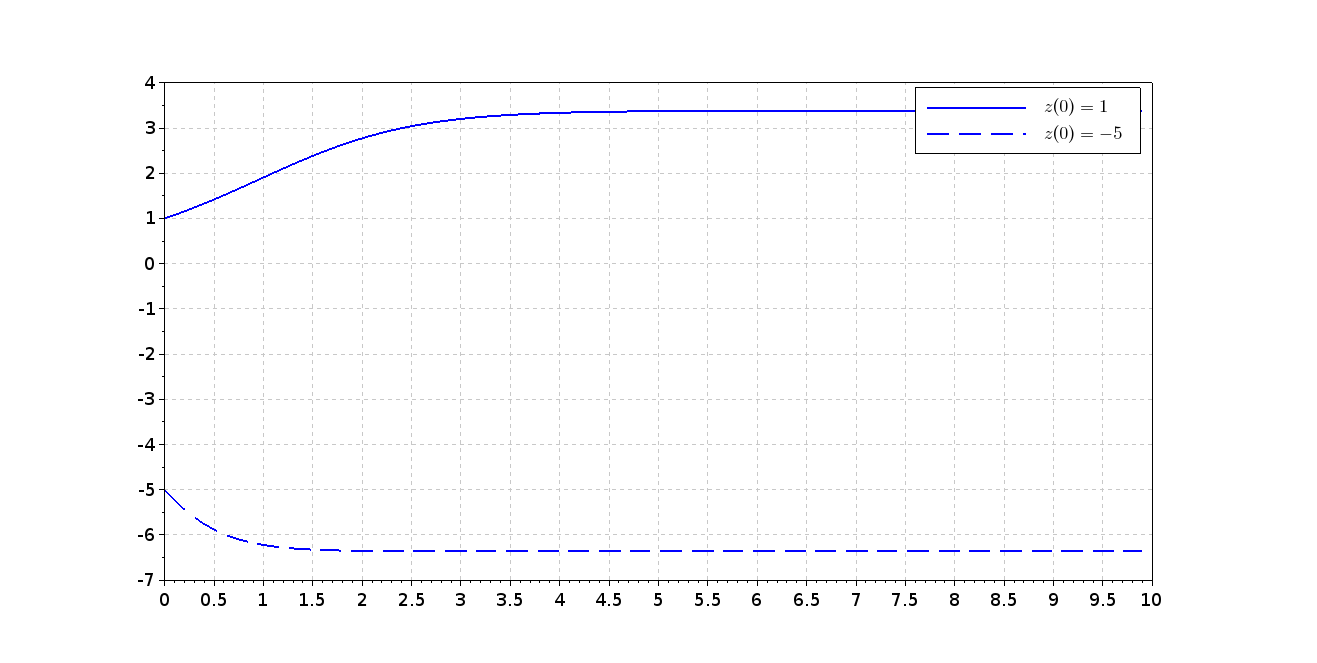
\includegraphics[width=1\textwidth]{graph2.png}
	\caption{Результаты моделирования}
	\label{aaa}
\end{figure}

В ходе выполнения домашней работы по курсу «Применение методов технического творчества в инновационной деятельности» был изучен патент SU 844986 \glqq Емкостной датчик микроперемещений\grqq, изложен принцип его действия, проанализирован с точки зрения основных законов развития технических систем (ТС), дан прогноз развития технической системы, синтезированы новые технические решения, выявлено техническое противоречие, которое затем было разрешено по АРИЗ, составлена статическая модель технического противоречия при помощи катастрофы типа сборки, получена динамическая модель, построен её фазовый портрет и получен переходный процесс.


\newpage